\documentclass[a4paper,12pt,twoside]{memoir}

% Castellano
\usepackage[spanish,es-tabla]{babel}
\selectlanguage{spanish}
\usepackage[utf8]{inputenc}
\usepackage[T1]{fontenc}
\usepackage{lmodern} % Scalable font
\usepackage{microtype}
\usepackage{placeins}
\usepackage{caption}

\RequirePackage{booktabs}
\RequirePackage[table]{xcolor}
\RequirePackage{xtab}
\RequirePackage{multirow}

% Links
\PassOptionsToPackage{hyphens}{url}\usepackage[colorlinks]{hyperref}
\hypersetup{
	allcolors = {red}
}

% Ecuaciones
\usepackage{amsmath}

% Rutas de fichero / paquete
\newcommand{\ruta}[1]{{\sffamily #1}}

% Párrafos
\nonzeroparskip

% Huérfanas y viudas
\widowpenalty100000
\clubpenalty100000

\let\tmp\oddsidemargin
\let\oddsidemargin\evensidemargin
\let\evensidemargin\tmp
\reversemarginpar

% Imágenes

% Comando para insertar una imagen en un lugar concreto.
% Los parámetros son:
% 1 --> Ruta absoluta/relativa de la figura
% 2 --> Texto a pie de figura
% 3 --> Tamaño en tanto por uno relativo al ancho de página
\usepackage{graphicx}

\newcommand{\imagen}[3]{
	\begin{figure}[!h]
		\centering
		\includegraphics[width=#3\textwidth]{#1}
		\caption{#2}\label{fig:#1}
	\end{figure}
	\FloatBarrier
}







\graphicspath{ {./img/} }

% Capítulos
\chapterstyle{bianchi}
\newcommand{\capitulo}[2]{
	\setcounter{chapter}{#1}
	\setcounter{section}{0}
	\setcounter{figure}{0}
	\setcounter{table}{0}
	\chapter*{#2}
	\addcontentsline{toc}{chapter}{#2}
	\markboth{#2}{#2}
}

% Apéndices
\renewcommand{\appendixname}{Apéndice}
\renewcommand*\cftappendixname{\appendixname}

\newcommand{\apendice}[1]{
	%\renewcommand{\thechapter}{A}
	\chapter{#1}
}

\renewcommand*\cftappendixname{\appendixname\ }

% Formato de portada

\makeatletter
\usepackage{xcolor}
\newcommand{\tutor}[1]{\def\@tutor{#1}}
\newcommand{\tutorb}[1]{\def\@tutorb{#1}}

\newcommand{\course}[1]{\def\@course{#1}}
\definecolor{newBox}{HTML}{D8AD6E}
\def\maketitle{
  \null
  \thispagestyle{empty}
  % Cabecera ----------------
\begin{center}
  \noindent
\includegraphics[width=\textwidth]{CabeceraEPS.png}\vspace{1.5cm}%
\end{center}
  
  % Título proyecto y escudo salud ----------------
  \begin{center}
    \begin{minipage}[c][1.5cm][c]{.20\textwidth}
        \includegraphics[width=\textwidth]{logo_GIS.png}
    \end{minipage}
  \end{center}
  
  \begin{center}
    \colorbox{newBox}{%
        \begin{minipage}{.8\textwidth}
          \vspace{.5cm}\Large
          \begin{center}
          \textbf{Necesidades del Paciente}\vspace{.6cm}\\
          \textbf{\LARGE\@title{}}
          \end{center}
          \vspace{.2cm}
        \end{minipage}
    }%
  \end{center}
  
    % Datos de alumno, curso y tutores ------------------
  \begin{center}%
  {%
    \noindent\LARGE
    Presentado por \@author{}\\ 
    en Universidad de Burgos\\
    \vspace{0.5cm}
    \noindent\Large
    \@date{}\\
    \vspace{0.5cm}

  }%
  \end{center}%
  \null
  \cleardoublepage
  }
\makeatother

\newcommand{\nombre}{Nicolás José García Gómez, Iván Mamolar Rupérez, Álvar Martínez Bailón y Pablo Santamaría Miguel}


% Datos de portada
\title{Dispositivo de detección de movimientos involuntarios en pacientes con parálisis cerebral ateoide}
\author{\nombre}
\date{\today}


\begin{document}

\maketitle



\frontmatter

% Abstract en castellano
\renewcommand*\abstractname{Resumen}
\begin{abstract}
Las afecciones neuromotoras, como la parálisis cerebral atetoide, se caracterizan por la presencia de movimientos involuntarios que dificultan tanto el control motor como la determinación de la voluntariedad de los movimientos. En este proyecto se propone una solución tecnológica orientada a la identificación y análisis de dichos movimientos.  

En primer lugar, se desarrolla una aplicación web denominada InvoluntTrack, que evalúa la capacidad del paciente para seguir trayectorias predefinidas mediante el cursor, registrando desviaciones interpretadas como posibles movimientos involuntarios y permitiendo obtener una representación visual y cuantitativa de posibles movimientos involuntarios. 

Complementariamente, se ha diseñado un prototipo de guante sensorizado basado en microcontroladores y sensores de distancia, fuerza e inclinación, que mide datos relacionados con el movimiento. A partir de la comparación entre patrones normales y patológicos, el sistema permite identificar desviaciones que puedan asociarse con determinadas enfermedades.
 
También se plantean líneas futuras de trabajo relacionadas con la integración de técnicas de análisis de datos y aprendizaje automático, así como el empleo remoto mediante plataformas de telemedicina. 

Este proyecto sienta las bases para el desarrollo de soluciones innovadoras en el ámbito del apoyo al diagnóstico y monitorización de trastornos motores. 


\end{abstract}

\renewcommand*\abstractname{Descriptores}
\begin{abstract}
Parálisis cerebral, parálisis cerebral atetoide, afecciones motoras, movimientos involuntarios, aplicación web, guante sensorizado. 
\end{abstract}

\clearpage

% Abstract en inglés
\renewcommand*\abstractname{Abstract}
\begin{abstract}
Neuromotor disorders, such as athetoid cerebral palsy, are characterized by the presence of involuntary movements that hinder both motor control and the ability to determine whether movements are voluntary. This project proposes a technological solution aimed at the identification and analysis of such movements. 

First, a web application called InvoluntTrack is developed, which evaluates the patient’s ability to follow predefined trajectories using a cursor. It records deviations that are interpreted as potential involuntary movements, providing both a visual and quantitative representation of these motor alterations. 

Additionally, a prototype of a sensorized glove has been designed, based on microcontrollers and distance, force, and inclination sensors, capable of measuring movement related data. By comparing normal and pathological patterns, the system enables the identification of deviations that may be associated with specific disorders. 

Future lines of work are also proposed, including the integration of data analysis and machine learning techniques, as well as remote usage through telemedicine platforms. 

This project lays the groundwork for the development of innovative solutions in the field of diagnostic support and monitoring of motor disorders. 

\end{abstract}

\renewcommand*\abstractname{Keywords}
\begin{abstract}
Cerebral palsy, athetoid cerebral palsy, motor impairments, involuntary movements, web application , sensorized glove. 
\end{abstract}

\clearpage

% Indices
\tableofcontents

\clearpage

\listoffigures

\clearpage

\listoftables
\clearpage


\mainmatter
\capitulo{1}{Introducción}


Las enfermedades neuromotoras engloban un conjunto de trastornos que afectan al control del movimiento, provocando en muchos casos la aparición de movimientos involuntarios. En pacientes que padecen este tipo de patologías, como la parálisis cerebral atetoide, una de las principales dificultades consiste en distinguir entre movimientos voluntarios e involuntarios. Esta diferenciación resulta fundamental tanto para la evaluación del paciente como para la interpretación de sus respuestas al interaccionar con diferentes profesionales. 

En este contexto, surge la necesidad de desarrollar herramientas que permitan analizar de la manera más objetiva posible los movimientos. El presente trabajo propone el diseño de soluciones tecnológicas orientadas a la detección y análisis de movimientos involuntarios, centrando su aplicación en pacientes con parálisis cerebral atetoide. Para ello, se abordan los conceptos teóricos de la patología y se plantean posibles soluciones que puedan facilitar la evaluación y detección de estos movimientos. 







\capitulo{2}{Objetivos}

La principal finalidad consiste en elaborar soluciones tecnológicas que permitan la identificación y análisis de movimientos involuntarios en pacientes con afectaciones neuromotoras, especialmente en parálisis cerebral atetoide. 

Entre los objetivos específicos se encuentran los siguientes: 
\begin{itemize}
    \item Analizar y comprender aspectos teóricos sobre la parálisis cerebral y a la parálisis cerebral atetoide 
    \item Diseñar una página web que permita detectar movimientos involuntarios en determinados pacientes. 
    \item Elaborar un prototipo de guante sensorizado que permita capturar y analizar datos relativos al movimiento. 
    \item Analizar posibles líneas futuras relacionadas que puedan implementarse en la práctica clínica. 
\end{itemize}










\capitulo{3}{Conceptos teóricos}


Este proyecto se centra principalmente en individuos que parecen un tipo específico de parálisis cerebral, la atetoide. Es necesario comprender los aspectos teóricos detrás de estas afecciones y sus características para poder desarrollar una solución tecnológica óptima y novedosa. 

\section{Conceptos teóricos básicos}
\subsection{¿Qué es la parálisis cerebral?}

La parálisis cerebral es un trastorno neuromotor crónico originado por una lesión o defecto durante el desarrollo del cerebro inmaduro causado durante un periodo comprendido entre los primeros días de gestación y los 5 años de vida \cite{MayoClinic2024}.

La denominación de “parálisis” nos da una gran información sobre las características de la enfermedad, y es que esta genera una gran debilidad y dificultad a la hora de utilizar los músculos, derivando en alteraciones motrices, del tono muscular y de la postura. No solamente afecta a la movilidad, sino que también causa problemas en otros aspectos como la cognición, derivando en déficit intelectual o dificultades en la comunicación \cite{GarciaRon2022, MedlinePlus2024}.

Entre las principales causas que la originan se encuentra la falta de flujo sanguíneo hacia el cerebro en el feto, alteraciones genéticas, infecciones por virus o bacterias, convulsiones o dificultades en el parto \cite{CentrodeNeurologaAvanzada2025}. 

\subsection{Tipos de parálisis cerebral}

Se pueden clasificar en función de la zona del cuerpo afectada:
\begin{itemize}
    \item Hemipléjica: afecta solo a una mitad del cuerpo, o la derecha o la izquierda.
    \item Paraplejia: afecta principalmente a todos los miembros inferiores.
    \item Tetraplejia: afecta a todas las extremidades, tanto a los miembros superiores como inferiores.
    \item Displejia: se ven afectadas las dos piernas, pero las extremidades superiores no se ven nada o casi nada afectadas.
    \item Monoplejia: cuando solo se ve afectado un miembro. 
\end{itemize}

En función de las características que presentan, podemos distinguir las siguientes:
\begin{itemize}
    \item Parálisis cerebral espástica: es la más común dándose entre un 60-70\% de los pacientes que padecen parálisis cerebral. Provoca rigidez y dificultad para controlar los músculos \cite{ASPACE, ASPACEGalicia2024}. 
    \item Parálisis cerebral atetoide: que provoca movimientos lentos, involuntarios y descoordinados. Deriva en problemas para controlar el movimiento de extremidades y en dificultades para estar sentado o caminando \cite{ASPACE, MedlinePlus2024}.
    \item Parálisis cerebral atáxica: afecta la coordinación y el equilibrio derivando en posturas y movimientos inestables \cite{eFISIO2023}. A pesar de las dificultades, existen personas que pueden llegar a caminar, aunque con muchas dificultades.
    \item Parálisis cerebral mixta: afecta a diferentes áreas cerebrales provocando una combinación de las dificultades mencionadas anteriormente en los otros tipos existentes.
\end{itemize}

Otra forma de clasificación es en función de si es leve, cuando se presentan alteraciones, pero no se ven limitadas las actividades diarias, moderada, cuando sí que existen dificultades en las actividades diarias y necesitan asistencia y apoyo, severa, cuando requiere ayuda para todas las actividades \cite{ASPACE}. También se pueden diferenciar en función del momento en el que aparece la lesión en prenatal, perinatal o postnatal \cite{ValldHebron2026}.


\subsection{Parálisis cerebral ateoitde}

Para este proyecto interesa la parálisis cerebral atetoide debido a sus característicos movimientos involuntarios, por lo que se va a profundizar en esta para comprender mejor con qué tipo de pacientes se trata.

También conocida como discinética, es el segundo tipo de parálisis más común presentándose entre el 10-15\% de personas con parálisis y requiere de terapia y asistencia de por vida \cite{PercyMartnez2025}. Se caracteriza por ser trastorno permanente no progresivo que se origina por una lesión cerebral que tiene lugar durante el desarrollo fetal o a lo largo de la primera infancia \cite{Li2022}. Su principal característica es que dificulta el control y coordinación muscular provocando movimientos involuntarios, que suelen afectar a los brazos las piernas o el rostro afectando a el desarrollo y la calidad de vida del paciente \cite{eFISIO2022}.

Su aparición se suele relacionar con los ganglios basales y lesiones talámicas que además pueden estar acompañadas de periodos hipóxicos breves. Una de las causas es kernicterus derivado de hiperbilirrubinemia neonatal provocando que la bilirrubina se acumule en los ganglios basales. Hoy en día la hiperbilirrubinemia se previene y trata con mayor eficacia por lo que ha disminuido la presencia de esta enfermedad, pero, aun así, sigue presente por vías como hemorragias intracraneales, ictus o infecciones de los ganglios basales o tálamo.

El tratamiento está enfocado en el control de los síntomas y la mejora de la calidad de vida del paciente. Para esto se emplean medicamentos para la reducción del dolor en caso de que haya y medidas para el tratamiento de los síntomas generalmente mediante la asistencia de un equipo integrado por profesionales clínicos, terapeutas y especialistas en salud conductual que tratan de maximizar la calidad de vida.

También existen medicamentos como el GABA-B, la estimulación cerebral profunda o la toxina botulínica que se pueden emplear pero que hasta el momento no han demostrado tener una gran eficacia \cite{Li2022}.

\section{Estado del arte y trabajos relacionados.}

Al llevar a cabo un proyecto en el que se aporta una solución tecnológica, es muy importante tener en cuenta qué se ha desarrollado hasta el momento para no repetirlo. El objetivo es aportar novedades que o bien creen soluciones completamente nuevas o mejoren las ya existentes.

\subsection{Wearable Devices for Assessment of Tremor}

Este artículo realiza una revisión sobre el creciente uso de los dispositivos wereables a la hora de evaluar el temblor en determinadas enfermedades. Se analizan los sensores inerciales, giroscopios y acelerómetros como medio de evaluar el movimiento de manera que puedan ser útiles a la hora de valorar la progresión de un trastorno como el Parkinson. 

Concluye que existen desafíos importantes a la hora de distinguir el temblor de otros movimientos involuntarios pero que este tipo de dispositivos tienen un gran potencial. \cite{Vescio2021}

\subsection{Wearable inertial sensors for human movement analysis: a five-year update}

Evalúa el empleo de sensores inerciales durante los últimos años como métodos de seguimiento cotidiano y prolongado. Presentan un gran potencial a la hora de analizar enfermedades neurológicas que generen alteraciones motoras por su capacidad para detectar patrones de movimiento. 

Su mayor reto está en ser capaces de elaborar algoritmos que interpreten de manera adecuada las señales que captan para poder dar una interpretación clínica fiable. \cite{Picerno2021}

\capitulo{4}{Aplicación web para la detección de movimientos involuntarios}

\section{Objetivo}

La aplicación \textbf{InvoluntTrack}, desarrollada en formato web, permite evaluar la capacidad del usuario para seguir una trayectoria lineal predefinida mediante el cursor del ratón. En condiciones normales, cuando el sistema nervioso motor funciona correctamente, el usuario es capaz de mantener el cursor dentro de los límites a lo largo de todo el recorrido. Por el contrario, si existe alguna lesión en el sistema nervioso que provoque la alteración del movimiento, se producirán desviaciones del cursor respecto a la trayectoria. La aplicación detecta y registra estas salidas, interpretándolas como posibles movimientos involuntarios.

El programa no pretende ser una herramienta de diagnóstico, sino un apoyo a la toma de decisiones clínicas permitiendo detectar patrones de movilidad involuntaria de forma rápida y visual.

El nombre de la aplicación surge de la combinación de dos conceptos. Por un lado, \textbf{"Involunt"}, abreviatura de involuntario, representando al tipo de movimientos que la aplicación pretende detectar. Por otro lado, \textbf{"Track"}, haciendo referencia a la trayectoria que realiza el usuario durante la prueba.
\clearpage
\section{Funcionamiento}
Al comenzar la prueba, aparece una trayectoria predefinida sobre un recuadro interactivo, con un punto de inicio y un punto de fin definidos. El usuario debe desplazar el cursor del ratón desde el inicio hasta el fin intentando mantenerlo dentro del tramo. Durante el recorrido, la aplicación detecta cualquier desviación, marcando y registrando los puntos donde se han producido las salidas. Al finalizar, se muestra un resumen de las salidas detectadas y una clasificación orientativa, además tiene la posibilidad de guardar la imagen que incluye tanto la trayectoria original como la seguida por el usuario, para posteriores análisis o elaboración de informes.

La aplicación tiene disponibles cuatro niveles de dificultad en función de la complejidad que se requiera para el usuario, desde una línea horizontal en el nivel más sencillo, hasta trayectorias con curvas y cambios bruscos de movimientos en los niveles más complejos. Esto permite adaptar la prueba a distintos perfiles en función del nivel de afectación del sistema nervioso.

\begin{center}
	    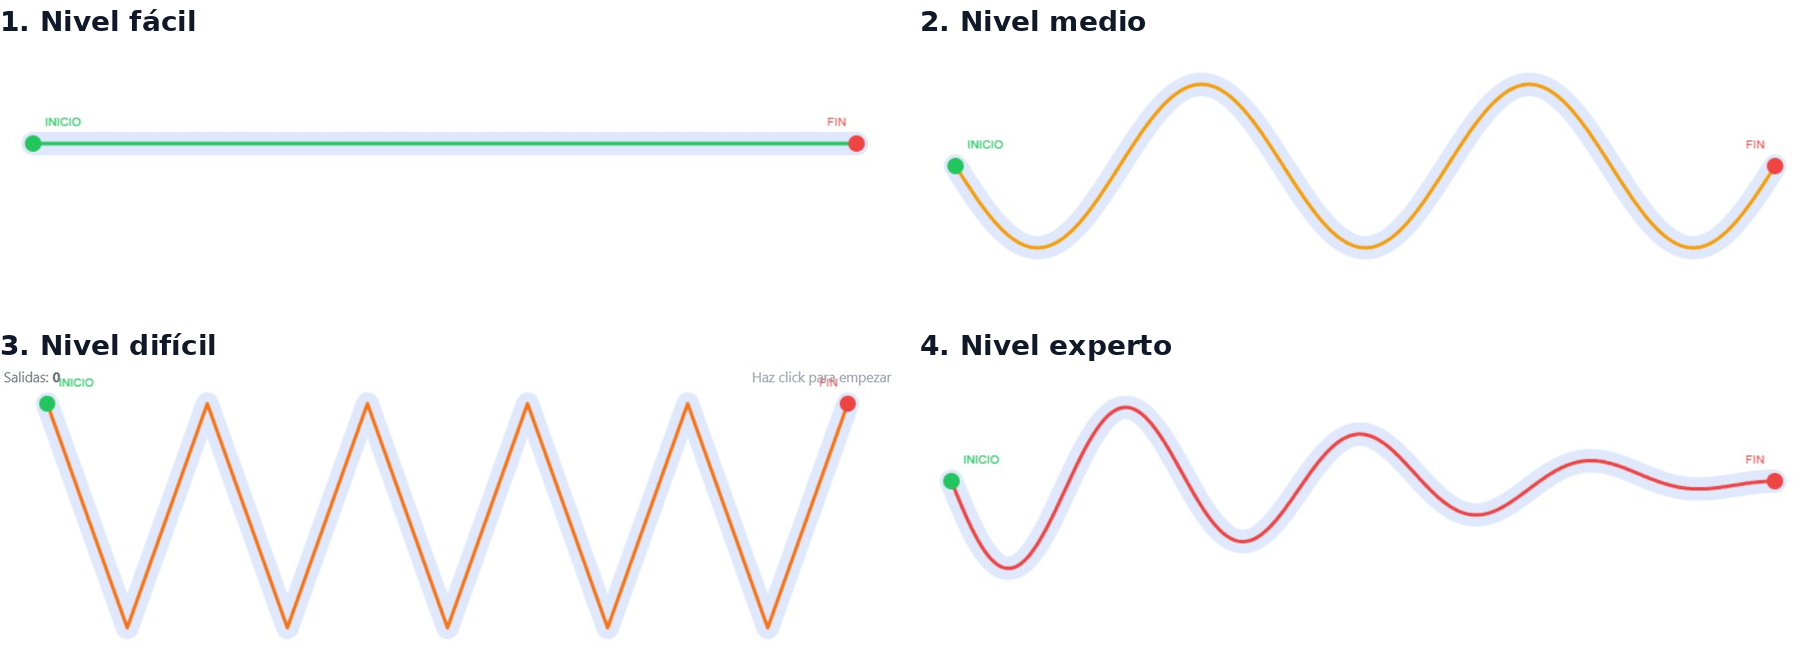
\includegraphics[width=1\textwidth]{img/niveles.png}
	    \captionof{figure}{Niveles disponibles en la aplicación.}
	    \label{fig:niveles}
	\end{center}

Además, la aplicación cuenta con un parámetro de tolerancia de error configurable por el usuario. Este parámetro, definido en pixeles, establece un margen de error alrededor de la trayectoria, funcionando como el límite máximo. Es decir, hasta que el usuario no traspasa el margen de error con el cursor, la aplicación no registra la salida. La tolerancia al igual que los niveles de dificultad, permite personalizar la prueba a cada usuario.
\clearpage
\section{Código}

La aplicación se ha desarrollado a través de Streamlit, aunque el funcionamiento central se encuentra en un bloque de HTML y JavaScript, contando principalmente con las siguientes funciones:


La función \textbf{buildPath()}, es la encargada de crear la trayectoria que el usuario debe seguir. Para ello, crea 500 puntos a lo largo del recuadro y según el nivel de dificultad seleccionado, varía la altura de cada punto para formar un tipo de línea u otro. 

En el caso de dificultad fácil, todos los puntos tienen la misma altura consiguiendo una línea recta, mientras que en los casos mas complejos se utilizan funciones matemáticas, como los senos para conseguir trayectorias con forma de ondas.

La función \textbf{ndist()} calcula la distancia mínima entre la posición del cursor y la trayectoria predefinida. Para ello, recorre los puntos que definen el camino y calcula la distancia de todos los puntos con el cursor y selecciona la menor, de esta forma el programa sabe dónde se encuentra el cursor durante el recorrido. 

La posición del cursor, se utiliza para determinar si el cursor se encuentra dentro o fuera de los límites, mediante la función \textbf{updateTrace()}. Esta función, compara la posición del cursor con el valor de tolerancia establecido. Si la posición es mayor que la tolerancia: se considera fuera, marca el punto de salida y registra la desviación en el contador de salidas. En caso contrario, la aplicación continua con el recorrido normal.

Es importante destacar que la aplicación registra solamente la primera salida de la trayectoria. Si el usuario se encuentra fuera del recorrido, no se contabilizan nuevas salidas hasta que el cursor vuelva a entrar dentro de los límites de la trayectoria y lo vuelva a superar. De esta forma, se tiene un recuento de las salidas y no del tiempo que el usuario pasa fuera.

Las funciones \textbf{startTrace()} y \textbf{finishTrace()}, se encargan del inicio y el final de la prueba. Cuando el usuario hace click en el recuadro, comienza a dibujar la trayectoria del cursor, hasta llegar al punto de fin, donde la prueba finaliza automáticamente. Cuando llega a este punto, también se desbloquean las opciones de ver resultados, guardar imagen o reiniciar prueba.

 La función \textbf{draw()} se encarga de la visualización de la prueba. Permite representar la trayectoria guía, la trayectoria del cursor del usuario, el margen de error de la tolerancia, así como los puntos donde el cursor supera los límites.

Por último, entre las funciones principales se encuentra \textbf{showResults()} que genera una interpretación orientativa en función del número de salidas:
	\begin{itemize}
	\item Número de salidas = 0 -> No hay movimientos involuntarios
	\item Número de salidas < 10 -> Posible afectación
	\item Número de salidas > 10 -> Afectación considerable
	\end{itemize}
	
Además cuenta con otras funciones como \textbf{saveImage()} que permite guardar la imagen con la trayectoria guía y la trayectoria generada por el usuario, o la función \textbf{resetCanvas()} que borra las trayectorias creadas y reinicia los contadores y resultados, permitiendo repetir la prueba.

\section{Interfaz}

La aplicación cuenta con una pantalla principal donde aparecen los siguientes elementos:

\subsection{Selección del nivel de dificultad:}
El usuario o personal médico responsable de realizar la prueba puede elegir a través de un desplegable el nivel de dificultad, en función de las características del usuario.

\begin{center}
	    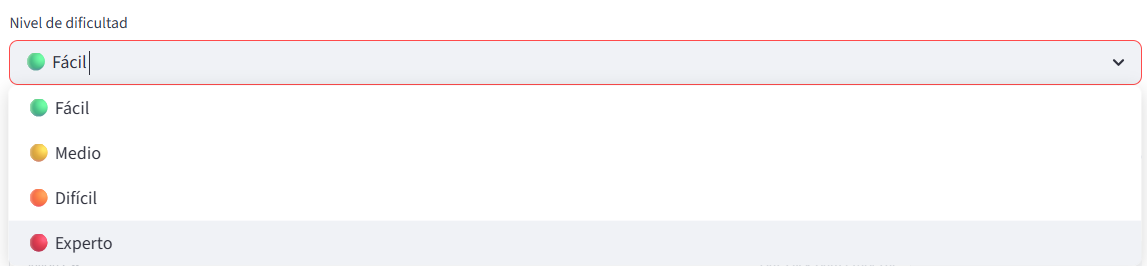
\includegraphics[width=0.9\textwidth]{img/nivel_dificultad.png}
	    \captionof{figure}{Selección de niveles de dificultad.}
	    \label{fig:selección_niveles}
	\end{center}
	
\subsection{Ajuste de tolerancia:}
La tolerancia se puede ajustar deslizando el indicador sobre la siguiente barra hasta obtener el valor correspondiente. Por defecto, todos los niveles tienen un nivel de tolerancia de 10 pixeles.

\begin{center}
	    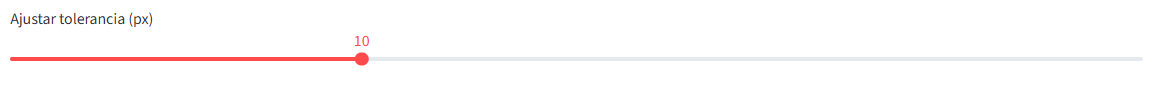
\includegraphics[width=1\textwidth]{img/tolerancia.png}
	    \captionof{figure}{Ajuste de tolerancia.}
	    \label{fig:selección_niveles}
	\end{center}
	
\subsection{Recuadro interactivo:}
Este recuadro permite al usuario dibujar la trayectoria guiándose del patrón predefinido. Cuando el usuario sobrepasa los límites establecido, la aplicación marca con un punto las zonas de salidas e incrementa el contador, obteniendo el número de desviaciones total.

\begin{center}
	    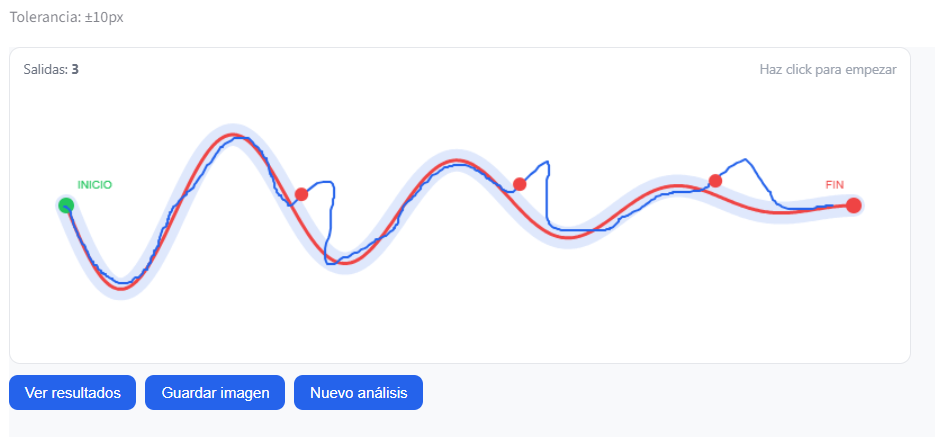
\includegraphics[width=0.55\textwidth]{img/prueba_trayectoria.png}
	    \captionof{figure}{Ejemplo de trayectoria (usuario).}
	    \label{fig:ejemplotrayectoria}
	\end{center}
	
Cuando el usuario llega al final de la trayectoria definida, aparecen tres botones que permiten:

\begin{itemize}
\item Ver los resultados de la prueba. Principalmente son estimaciones que pueden ayudar al diagnóstico, por lo que el personal médico que realice la prueba es el encargado de interpretarlos y considerar si son válidos para el diagnóstico final:

\begin{center}
	    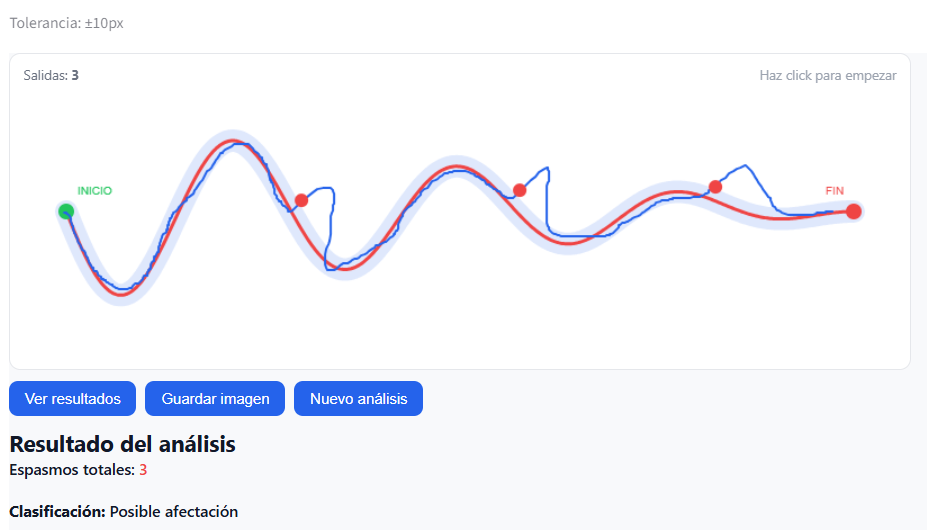
\includegraphics[width=0.7\textwidth]{img/resultados.png}
	    \captionof{figure}{Resultados de ejemplo.}
	    \label{fig:resultados}
	\end{center}

\item Guardar la imagen de la trayectoria realizada por el usuario junto a la trayectoria guía:
\begin{center}
	    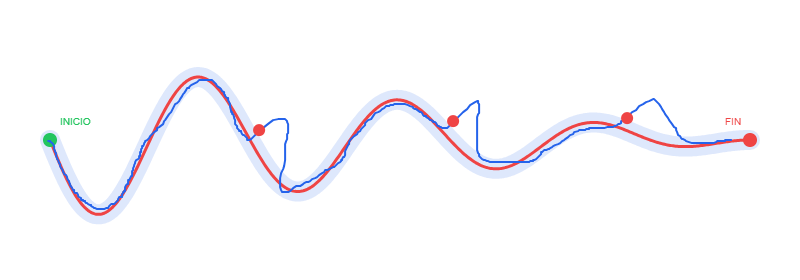
\includegraphics[width=0.7\textwidth]{img/trayectoria_guardada.png}
	    \captionof{figure}{Trayectoria guardada.}
	    \label{fig:guardado}
	\end{center}

\item Por último, reiniciar la prueba, limpiando las trayectorias realizadas y poniendo a cero todos los contadores

\subsection{Interfaz global:}

\begin{center}
	    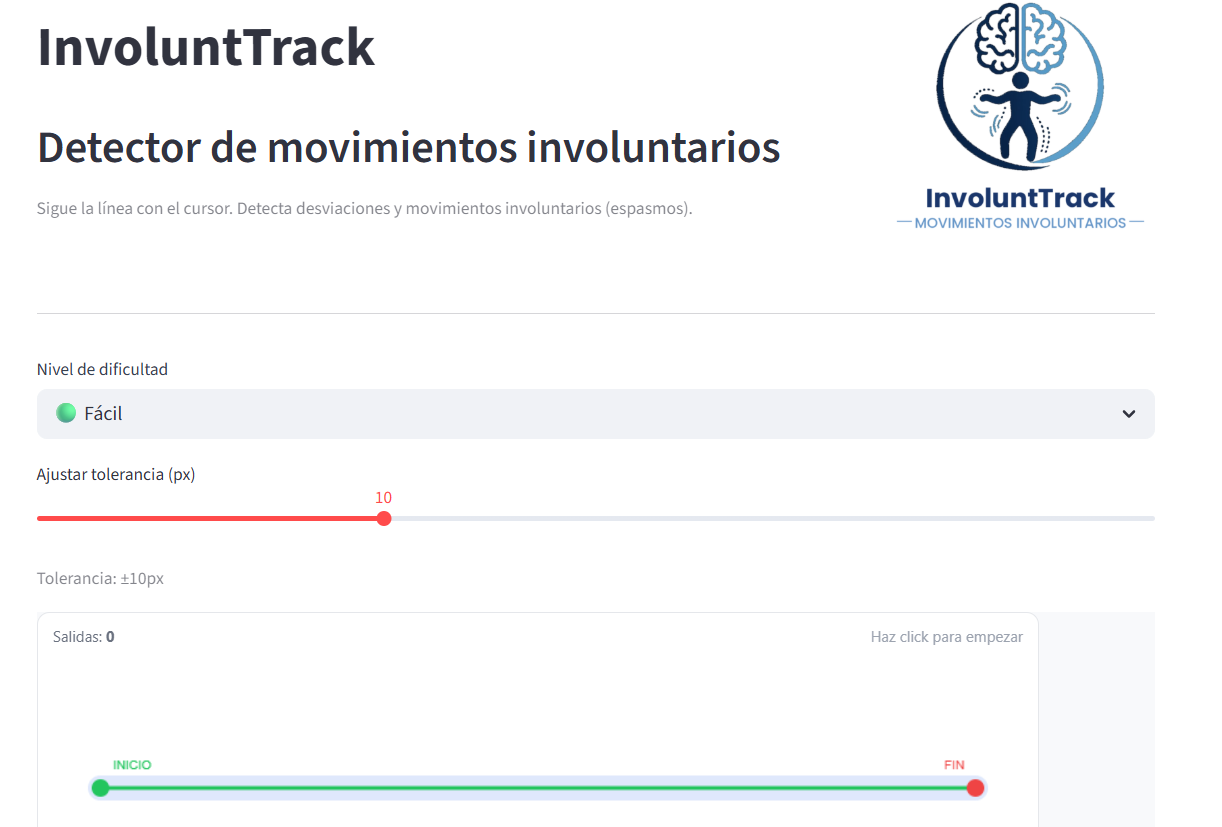
\includegraphics[width=1\textwidth]{img/interfaz_global.png}
	    \captionof{figure}{Interfaz global.}
	    \label{fig:interfaz}
	\end{center}

\end{itemize}

\clearpage
\section{Posibles mejoras}

La aplicación desarrollada es un prototipo funcional cuyo objetivo es demostrar el funcionamiento del programa propuesto para la detección de movimientos involuntarios. Por este motivo, presenta aspectos que pueden ser mejorados para aumentar la precisión, funcionalidad y accesibilidad.

\begin{itemize}
\item Emplear distintos sistemas de entrada, como pantallas táctiles o tablets, que permitan simular situaciones de movimiento más realistas y faciliten la adaptabilidad a usuarios que no puedan manejar el ratón.
\item Crear trayectorias más complejas y aleatorias para que los usuarios no se adapten a los mismos recorridos
\item Implementar nuevas pruebas que permitan detectar otros tipos de afectaciones neurológicas.
\item Incorporar nuevas métricas como velocidad del cursor, cambios bruscos de dirección o intensidad de temblor.
\item Utilizar clasificaciones más representativas, validadas por expertos neurológicos.
\item Añadir un sistema de usuarios que permita guardar la información de distintos pacientes, las pruebas realizadas, informes, trayectorias ...

\end{itemize}

\section{Presupuesto}

El presupuesto aproximado para el desarrollo de la aplicación web se ha calculado teniendo en cuenta tanto la parte hardware como software necesarias, así como el coste asociado al trabajo del personal técnico.

En cuanto al hardware, ha sido necesario principalmente un equipo informático ya sea portátil o de sobremesa, incluyendo sistemas de entrada de información claves para el funcionamiento de la aplicación como el ratón del ordenador.
\clearpage
\begin{itemize}
\item \textbf{Ordenador portátil:} se toma como referencia el modelo de portátil utilizado durante el desarrollo del trabajo. Consiste en un ordenador HP con procesador \textit{intel core i7} y dispone de la versión \textit{windows 11}, cuyo precio ronda los 780 € \cite{hp_15_fd0334ns_pccomponentes}. Aunque existen otras opciones más económicas igualmente válidas.
\item \textbf{Ratón (mouse):} los precios de estos dispositivos rondan en torno a los 10-13€ \cite{conceptronic_regas_tw5_pccomponentes}, por lo que esta decisión dependerá del usuario que vaya a utilizar la aplicación siempre y cuando sea funcional.
\end{itemize}

Respecto a la parte software, la aplicación se ha desarrollado a través de la librería de Python Streamlit junto a otros lenguajes como JavaScript y HTML. Estas herramientas son de acceso libre y no requieren el uso de licencias de pago, por lo que esta parte del desarrollo no supone ningún coste económico adicional.

Por otro lado, se incluyen los costes personales que suponen el desarrollo de la aplicación, estimado en base al sueldo medio de un ingeniero biomédico/de la salud junior que ronda entre los 25000€ y 35000€ anuales \cite{ufv_biomedico_salario_espana}, lo que se traduce a aproxiamdamente 2000€-2500€ mensuales. Al tratarse de un proyecto desarrollado por un equipo de cuatro personas, este coste se ha tenido en cuenta considerando la colaboración conjunta de todos los integrantes del grupo, multiplicando este valor por cuatro.

\begin{table}[h]
\centering
\begin{tabular}{|l|l|l|}

\hline
\rowcolor{gray!20}
\textbf{Concepto} & \textbf{Descripción} & \textbf{Coste estimado} \\ \hline
Hardware & Ordenador portátil & 780 € aprox. \\ 
Hardware & Sistemas de entrada (ratón) & 13 € aprox. \\ \hline
Software & Streamlit, JavaScript, HTML (software libre) & 0 € \\ \hline
Personal (1 persona) & Ingeniero biomédico junior (mensual) & 2000 € -- 2500 € \\ 
Personal (4 personas) & Equipo de desarrollo (mensual) & 8000 € -- 10000 € \\ \hline
\rowcolor{yellow!30}
\textbf{Total estimado} &  & \textbf{8793 €} \\ \hline
\end{tabular}
\caption{Presupuesto del proyecto}
\label{tab:presupuesto}
\end{table}
\capitulo{5}{Guante de detección de movimientos involuntarios}

\section{Objetivos}
Uno de los principales inconvenientes de este tipo de patologías es su diagnóstico.
Muchos de estos movimientos son tan imperceptibles o se parecen tanto unos a otros que se hace prácticamente imposible su diagnóstico, impidiendo que los médicos y rehabilitadores sepan con claridad que tipo de tratamiento o terapia seguir y haciendo que su complicada clínica sea aún más difícil.

En un contexto médico donde cada vez se busca más la especialización y la individualización de cada paciente, se ha creado una herramienta que  permitirá obtener datos muy valiosos para ser mucho más específicos en el diagnóstico.

Habiendo explicado todo lo que se sabe a día de hoy sobre los movimientos involuntarios, su principal inconveniente es el diagnóstico, y tras recoger los datos sobre los patrones de movimientos voluntarios e involuntarios mediante la simple prueba del ratón de la aplicación web antes mencionada, se ha conseguido implementar una posible solución para el diagnóstico.

\clearpage

\section{Componentes}

Esta solución consta de un guante el cual hay que modificar con el fin de poder ajustar una serie de sensores situados en una estancia o cubículo que permiten medir el movimiento. Dichos sensores son la clave y el corazón de esta herramienta que a continuación describiremos junto con el resto de componentes:

\begin{itemize}
    \item \textbf{Sensores de distancia ultrasónicos:} Estos se encuentran situados en el cubículo o caja para hacernos más a la idea y permiten conocer la distancia a la que se encuentra la mano de las paredes.
    \item \textbf{Sensor de fuerza:} Permite saber la fuerza que aplica la mano en el guante.
    \item \textbf{Sensor de inclinación:} Nos permite conocer la inclinación que tiene la mano.
    \item \textbf{Arduino:} Es el microcontrolador de la herramienta la cual, nos permite cargar y guardar datos sobre el paciente.
    \item \textbf{Pantalla LCD:} Simplemente es una pantalla que permita al médico ver de manera rápida que sensor es el que está capturando movimientos anómalos.
    \item \textbf{Leds:} Es un refuerzo aun más visual al de la pantalla LCD. 
    \item  \textbf{Protoboards:} La pequeña simula el guante del paciente y la grande seria la caja exterior.
\end{itemize}

\section{Metodología}

Como ya hemos explicado anteriormente esta herramienta es básicamente un guante que consta de una serie de sensores y se encuentra situado en una caja que cuenta con sus propios sensores. 

Gracias a los datos obtenidos de la aplicación anterior, se han trackeado los parámetros de diferentes personas sin ningún tipo de patología generando un mapa “normal” y de personas con las diferentes patologías mencionadas y ya diagnosticadas, generando a su vez un mapa problemático de cada una de las patologías.

Una vez obtenidos estos dos mapas, el “normal” y el problemático, hay que compararlos. Esto permite saber que en una patología especifica el movimiento involuntario se caracteriza, por ejemplo, con una fuerza de 100N y una desviación lateral predominante hacia la izquierda.

Esto es un avance muy significativo a la hora del diagnóstico, ya que permite saber de manera específica y cuantitativa, cuáles son los parámetros que varían de las personas sin patología para cada una de las enfermedades estudiadas. Los pasos a partir de ahora son muy simples:

\begin{enumerate}
    \item Una vez obtenidos estos parámetros anormales se introducen en el microcontrolador del guante, por ejemplo:
	\begin{itemize}
		\item Una inclinación máxima de 30\textdegree.
		\item Una fuerza máxima de 75 N.
		\item Una desviación predominante hacia la derecha.
	\end{itemize}
    \item La persona por examinar se pone el guante con los parámetros cargados de la patología que se quiere diagnosticar, situándose dentro de la caja con sensores de distancia.
    \item Se le realizan una serie de preguntas a las que responder y se deja un tiempo la mano inmóvil.
    \item Los datos recogidos por los sensores son comparados en el microcontrolador con los datos que hemos cargados.
    \item Por la pantalla aparece si alguna de las características de la enfermedad ha aparecido, permitiendo saber si los datos cargados de la patología concuerdan con los captados del paciente.
\end{enumerate}

\section{Diseño de prototipo}

El diseño que se ha desarrollado en \textit{Tinkercad} está constituido por tres componentes principales que son los encargados de proporcionar las funcionalidades especificadas:

\begin{itemize}
	\item Tres sensores de distancia, que en conjunto representan el perímetrod e la caja. Cada uno de ellos se ve como en la Figura \ref{fig:sensdistancia}.  

	\begin{center}
	    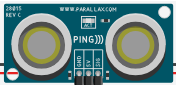
\includegraphics[width=0.4\textwidth]{img/Sensor_distancia.png}
	    \captionof{figure}{Sensor de distancia del guante.}
	    \label{fig:sensdistancia}
	\end{center}

	\item Sensores de fuerza e inclinación, que se visualizan en la Figura \ref{fig:sensfuerzainc}. 

	\begin{center}
	    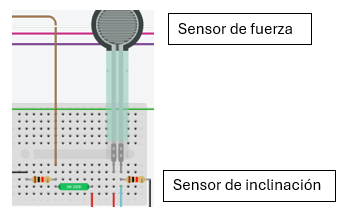
\includegraphics[width=0.6\textwidth]{img/Sensor_fuerza_inclinacion.png}
	    \captionof{figure}{Sensores de fuerza e inclinación.}
	    \label{fig:sensfuerzainc}
	\end{center}
\end{itemize}

El diseño completo del circuito final se puede apreciar en la Figura \ref{fig:guante}. 
\begin{center}
    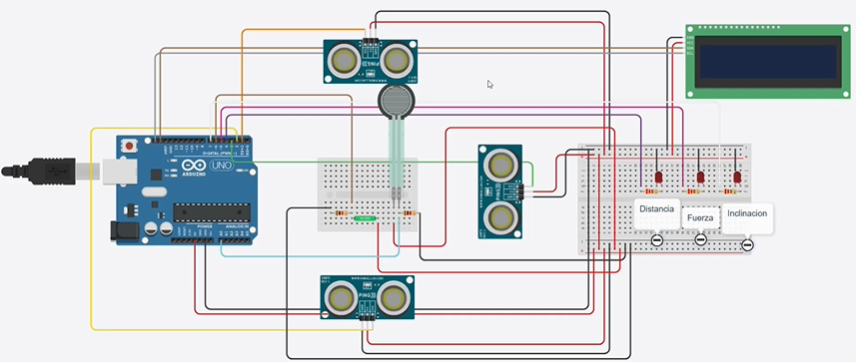
\includegraphics[width=0.9\textwidth]{img/Guante_tinkercad.png}
    \captionof{figure}{Diseño de  \textit{Tinkercad} del guante de detección movimiento involuntarios.}
    \label{fig:guante}
\end{center}


\section{Funcionamiento}
Una vez en funcionamiento, cada vez que la mano excede los límites de los sensores de la caja, la pantalla muestra un mensaje de advertencia que depende cual sea, pone izquierda, derecha o arriba.

También muestra las posibles combinaciones de coincidencias con los datos cargados, como puede ser distancia con fuerza, distancia con inclinación, inclinación con fuerza y muestra un mensaje total cuando se presentan los tres tipos de coincidencias.

Obviamente cuando no se da ningún tipo de coincidencia entre los datos de los sensores y los cargados, la pantalla muestra un mensaje anunciando que todos los valores son correctos.


\section{Presupuesto}
Por último, en la Figura \ref{fig:presguante} ,se ve el presupuesto simplificado del coste de creación y desarrollo de esta herramienta en concreto.
\begin{center}
    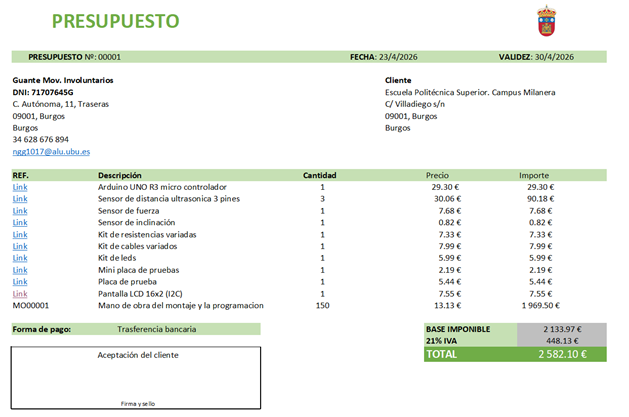
\includegraphics[width=1.0\textwidth]{img/Presupuesto_guante.png}
    \captionof{figure}{Presupuesto del guante de detección de movimientos involuntarios.}
    \label{fig:presguante}
\end{center}
\capitulo{8}{Lineas de trabajo futuras}


Como continuación del presente trabajo, se propone el desarrollo de una línea de investigación orientada a la evolución del sistema hacia una plataforma híbrida que combine análisis cualitativo y cuantitativo del movimiento. En este sentido, uno de los principales avances consistiría en la incorporación de un módulo de validación cuantitativa basado en la obtención de parámetros numéricos objetivos derivados de los datos capturados por el guante sensorizado.

Dicho módulo permitiría transformar las señales recogidas (posición, velocidad, aceleración y orientación) en indicadores medibles, tales como amplitud de movimiento, velocidad angular, frecuencia de ejecución, estabilidad y simetría entre extremidades. Estos parámetros podrían calcularse mediante la aplicación de modelos matemáticos y físicos básicos, como derivadas temporales para el cálculo de velocidad y aceleración, o métricas estadísticas para evaluar la variabilidad del movimiento. La integración de estos valores facilitaría la comparación con rangos de normalidad previamente definidos en función de la edad y el desarrollo motor del paciente, contribuyendo así a una evaluación más objetiva y reproducible.

Además, la incorporación de técnicas de análisis de datos y aprendizaje automático permitiría identificar patrones característicos asociados a posibles alteraciones neuromotoras, mejorando la capacidad del sistema para apoyar la detección temprana. En esta línea, resulta especialmente relevante el desarrollo de modelos personalizados que se adapten a las características individuales de cada paciente, teniendo en cuenta su evolución a lo largo del tiempo. El uso de datos longitudinales permitiría no solo detectar desviaciones puntuales, sino también analizar tendencias y progresión de la patología, aportando un valor significativo en el seguimiento clínico.

Por otra parte, se plantea como mejora del dispositivo hardware el diseño de un guante inteligente que integre una pantalla o interfaz visual embebida. Esta pantalla permitiría proporcionar retroalimentación en tiempo real tanto a profesionales sanitarios como a los propios usuarios. A nivel clínico, se podrían mostrar métricas relevantes, alertas ante desviaciones significativas y representaciones gráficas simplificadas de la evolución del paciente. Desde la perspectiva del usuario, especialmente en el caso de niños, la interfaz podría ofrecer indicaciones visuales intuitivas, refuerzo positivo y elementos de gamificación que favorezcan la adherencia al uso del sistema.

Adicionalmente, se propone la integración del sistema con plataformas de telemedicina, lo que permitiría la monitorización remota de los pacientes y el acceso a los datos por parte de profesionales sanitarios en tiempo real. Esta funcionalidad facilitaría la continuidad asistencial, reduciría la necesidad de desplazamientos y ampliaría el alcance del sistema a entornos domiciliarios o rurales.

Finalmente, la combinación de estos avances abriría la puerta a nuevas aplicaciones, como el seguimiento longitudinal de pacientes, la monitorización remota y el uso del sistema como herramienta de apoyo en procesos de rehabilitación. En conjunto, estas líneas de investigación contribuirían a mejorar la precisión, usabilidad y aplicabilidad clínica del sistema propuesto, consolidándolo como una herramienta innovadora en el ámbito de la evaluación y apoyo al diagnóstico de alteraciones neuromotoras.




\bibliographystyle{apalike}
\bibliography{bibliografia}

\end{document}
